\documentclass[12pt]{standalone}
\usepackage[english]{babel}
\usepackage[utf8]{inputenc}

\usepackage{comment}
\usepackage{amsmath}
\usepackage{tikz}
\usepackage{circuitikz} 
\usetikzlibrary{arrows.meta} 
\usetikzlibrary{positioning}
\usetikzlibrary{calc}

\newcommand\ppbb{path picture bounding box}
\tikzset{
  do path picture/.style={%
    path picture={%
      \pgfpointdiff{\pgfpointanchor{\ppbb}{south west}}%
        {\pgfpointanchor{\ppbb}{north east}}%
      \pgfgetlastxy\x\y%
      \tikzset{x=\x/2.5,y=\y/2.5}%
      #1 }
  },
  sin wave/.style={do path picture={    
    \draw [line cap=round] (-3/4,0)
      sin (-3/8,1/2) cos (0,0) sin (3/8,-1/2) cos (3/4,0); }
  },
	gen/.style={circle, draw=black, thick, minimum width = 2em,sin wave},
	infGen/.style={ circle, draw=black, thick, minimum width = 2em, },
}

\begin{document}
% create tikz environment, configure cicuitikz
	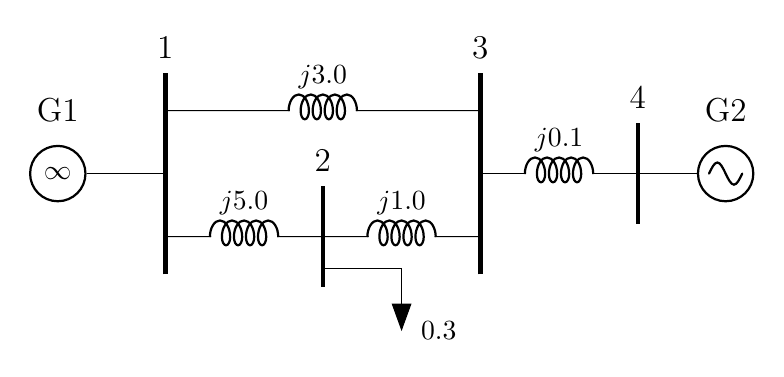
\begin{tikzpicture} [american voltages,scale=.8, 
		breaker/.style={rectangle,draw=black,fill=white},
		load/.style={-{Triangle[length=3.5mm,width=2.5mm,open,fill=black]}},
		node distance = 2 cm and 2 cm]
		
		% create gen 1 (infinite bus)- used as relative postiiton start point
		\node[infGen] (Igen) { $\infty$};
		
		% create bus coordinates
		\coordinate[right = 1cm of Igen](bus1) {};
		\coordinate[right  = 5 cm  of Igen](bus3) {}; % double spaced
		\coordinate[right = of bus3](bus4) {};
		
		% position bus 2 shifted down and centered between bus 1 and 3	
		\newcommand{\loadBusShift}{ -1.0 } % create 'variable' for load bus y shift
		\coordinate (bus2) at ($ (bus1) !0.5! (bus3) + (0,\loadBusShift) $)  {};
		
		% Draw generator 2
		\node[gen, right = .75 cm of bus4] (G1) {};
		
		% Label Generators
		\draw ($(Igen)+(0,1)$) node {\large G1};
		\draw ($(G1)+(0,1)$) node {\large G2};
		
		% Draw Load
		\node (load1) at ($(bus2) !0.5! (bus3) + (0,2*\loadBusShift)$) [label=0:0.3]  {} ; %[label={[label distance=1cm]30:label}] 
		\draw[load] ($(bus2)+(0,-.5)$) -| ($(load1)$);
		
		% draw and label single length Vertical buses
		\foreach \busNum in {2, 4}
		{
			\draw[ultra thick] ([yshift=-0.8cm]bus\busNum.south) -- ([yshift=+0.8cm]bus\busNum.north);
			\draw ($(bus\busNum) +(0,+1.2)$) node {\large{\busNum}};
		}
		
		% draw ane label double length Vertical buses
		\foreach \busNum in {1,3}
		{
			\draw[ultra thick] ([yshift=-1.6cm]bus\busNum.south) -- ([yshift=+1.6cm]bus\busNum.north);
			\draw ($(bus\busNum) +(0,+2.0)$) node {\large{\busNum}};
		}
		
		% Draw system Lines
		\draw (Igen) -- (bus1); % Line from Inf Bus to System
		\draw ($ (bus1) -(0,\loadBusShift) $) to [L, l= $j3.0$] ($ (bus3) - (0, \loadBusShift) $) ; %  top line
		\draw ($ (bus1) +(0,\loadBusShift) $) to [L, l= $j5.0$] (bus2) ; % 1-2 line
		\draw  (bus2) to [L, l= $j1.0$] ($ (bus3) +(0,\loadBusShift) $) ; % 2-3 line
		\draw (bus3) to [L, l= $j0.1$] (bus4); % 3-4 line
		\draw (bus4) -- (G1); % line to gen2 from bus 4

		
	\end{tikzpicture}

\end{document}